\documentclass[12pt,a4paper]{article}

\newcommand{\TETELNUMBER}{22}
\newcommand{\TETELTITLE}{Számítógép-hálózatok alapfogalmai és az ISO--OSI modell}
\newcommand{\TETELSHORTTITLE}{Hálózati alapfogalmak és OSI}

\newcommand{\ZVTetelsorDataOnly}{}
\newcommand{\ZVTetelOne}{Adatok, adattípusok, adatműveletek és adatstruktúrák. Szám adattípus. Számrendszerek, konverziók. A logikai, halmaz, karakter, sztring absztrakt adattípusok és realizációjuk. A tömb (vektor, mátrix), rekord absztrakt adattípusok.}
\newcommand{\ZVTetelTwo}{Az algoritmus. Iteratív és rekurzív algoritmus. A számítógépes memória. Adat és program. Verem és procedúra. Az algoritmus lejegyzése. A folyamatábra és a pszeudokód. Elemi algoritmusok.}
\newcommand{\ZVTetelThree}{Strukturált programozás. Programgráf, valódi program, vezérlőgráf lebontása, strukturált program és annak formulája. Strukturált programgráf kialakítása, struktogram. Ciklikus bonyolultság és egyéb bonyolultsági tételek.}
\newcommand{\ZVTetelFour}{Számelméleti algoritmusok. Legnagyobb közös osztó, euklideszi és kibővített euklideszi algoritmus, lineáris kongruencia egyenletek. Multiplikatív inverz, moduláris hatványozás, Fermat prímteszt. RSA.}
\newcommand{\ZVTetelFive}{Rendezések: Beszúró rendezés. Az ,,Oszd meg és uralkodj!'' elv. Összefésülő rendezés. Gyors rendezés. Buborék rendezés. Shell rendezés. Minimum kiválasztásos rendezés. Négyzetes rendezés. Lineáris idejű rendezések: leszámláló rendezés, számjegyes rendezés. Időelemzéseik. Az összehasonlító rendezések időtétele.}
\newcommand{\ZVTetelSix}{Gráfalgoritmusok. Szélességi keresés. Mélységi keresés. Topologikus rendezés. Optimumfeladatok fákon (minimális feszítőfák, Kruskal- és Prim-algoritmus). Legrövidebb utak meghatározása (Dijkstra-algoritmus, Bellman--Ford-algoritmus, Floyd--Warshall-algoritmus).}
\newcommand{\ZVTetelSeven}{A párhuzamos algoritmusok alapfogalmai, PRAM modell, hatékonysági mértékek (munka, költség, gyorsítás, hatékonyság). Párhuzamos végrehajtás ábrázolási módjai. Komplexitás becslése, párhuzamos komplexitás. Amdahl törvénye. Pipeline párhuzamosítás, Lost update probléma bemutatása és megoldása.}
\newcommand{\ZVTetelEight}{Aggregáció, redukció, prefixszámítás párhuzamosítási lehetőségei. \texttt{CREW\_PREFIX}, \texttt{EREW\_PREFIX} és \texttt{OPTIMAL\_PREFIX} algoritmusok bemutatása. Összefésülő rendezés párhuzamosítási módja.}
\newcommand{\ZVTetelNine}{A busz, gyűrű, rács, tórusz, hiperkocka és fa topológiák bemutatása, csomópontok közötti távolságok jellemzése. A CSP, Publish--Subscribe és az Aktor modell. Az aszinkron programozás elemei: async, await kulcsszavak használata, coroutine-ok.}
\newcommand{\ZVTetelTen}{A Turing-gép fogalma, működése. A RAM-gép. Boole-függvények és logikai hálózatok.}
\newcommand{\ZVTetelEleven}{Algoritmikus eldönthetőség. Church-tézis. Rekurzív és rekurzívan felsorolható nyelvek, rekurzív illetve parciálisan rekurzív függvények. Nevezetes nyelvek (Az R, Re, coR, coRE nyelvosztályok és ezek kapcsolata) és bonyolultságuk. Algoritmikusan eldönthetetlen problémák. Polinomiális idejű algoritmusok.}
\newcommand{\ZVTetelTwelve}{Nemdeterminisztikus Turing-gépek, az NP és a coNP nyelvosztály. Példák NP-beli nyelvekre. A tanú-tétel. Nemdeterminisztikus algoritmusok bonyolultsága. NP-teljesség, Cook-tétel. Néhány NP-teljes probléma, Cook--Levin-tétel.}
\newcommand{\ZVTetelThirteen}{A Java programozási nyelv története, alapvető jellemzői. Egy Java program szerkezete (csomagok és fordítási egységek). Az objektumorientált programtervezés alapelveinek felsorolása. Objektumok tárolása és élettartama. Szemétgyűjtő mechanizmus. Kivételkezelés.}
\newcommand{\ZVTetelFourteen}{Az egységbezárás és az információrejtés objektumorientált alapelvek megvalósítása. Osztálydefiníció és példányosítás. Osztályszintű és példányszintű tagok, konstansok. Hozzáférési kategóriák és használatuk. Hivatkozás az osztály tagjaira.}
\newcommand{\ZVTetelFifteen}{Az öröklődés és a polimorfizmus objektumorientált alapelvek megvalósítása. Öröklődés szabályai, metódusok túlterhelése és felüldefiniálása. A referencia statikus és dinamikus típusa. Absztrakt osztály és interfész szerepe, összehasonlítása.}
\newcommand{\ZVTetelSixteen}{Az operációs rendszerbeli folyamat (processz) fogalma. Folyamatkontextus. A fonál (szál) fogalma. A processzállapotok, állapotváltások, processz futási módok. Taszk- és fonálállapotok, állapotátmenetek.}
\newcommand{\ZVTetelSeventeen}{A memóriamenedzselés feladatai. Memória mint erőforrás. Címleképzés fajtái. Lapozós virtuális memóriamenedzselés működése. Allokálás, nyilvántartás, címleképzés. Laphiba fogalma, kezelése, kilapozási stratégiák. Előnyök, hátrányok.}
\newcommand{\ZVTetelEighteen}{Fájlrendszer-megvalósítási feladatok. Jegyzékszerkezetek. Szabadblokk-menedzselési lehetőségek. Fájlattribútum-rögzítési lehetőségek (ezen belül a fájltestet képező blokkok rögzítési lehetőségei).}
\newcommand{\ZVTetelNineteen}{Relációs adatmodell, relációs struktúra és integritási feltételek. ER modell elemei jelentése és jelölése. Az ER modell konverziója relációs modellre. Relációs adatmodell műveleti része, relációs algebra.}
\newcommand{\ZVTetelTwenty}{Az SQL szabvány relációs adatbázis kezelő nyelv bemutatása, a DDL (objektum létrehozás, megszüntetés és szerkezet módosítás), DML (rekord felvitel, törlés és módosítás), DCL és a SELECT utasítások áttekintése és használata. Beágyazott SELECT használata. A relációs algebra műveleteinek megvalósítása SQL-ben.}
\newcommand{\ZVTetelTwentyOne}{Adatkezelés és adatbáziskezelés alapfogalmai, fileszervezési módszerek, B-fa index; adatbázis architektúra; A normalizálás szerepe a relációs adatbázis kezelésben. Redundancia oka és a megszüntetés lépései. Normálformák. Dekompozíció célja és szabályai, tételei.}
\newcommand{\ZVTetelTwentyTwo}{Számítógép-hálózatokhoz kötődő alapfogalmak és az ISO--OSI hivatkozási modell: topológia és méret szerinti osztályozásuk. Kapcsolástechnika szerinti osztályozásuk (vonalkapcsolás, üzenetkapcsolás, csomagkapcsolás és virtuális vonalkapcsolás). Az ISO--OSI hivatkozási modell szerkezete, rétegei és azok főbb funkciói.}
\newcommand{\ZVTetelTwentyThree}{A számítógép-hálózatok ISO--OSI hivatkozási modell adatkapcsolati rétegének közeghozzáférési alrétege: A főbb csatorna-megosztási osztályok (statikus-dinamikus, dinamikus versengő-determinisztikus) bemutatása és azok összevetése. Az IEEE 802.3 és az Ethernet (CSMA/CD) keretformátum, MAC címek, támogatott közegek és sebességek bemutatása, működés duplex csatorna esetén. Az IEEE 802.11 WLAN általános felépítése, az Access Point (AP) főbb funkciói. Az alkalmazott közeghozzáférési módszer (CSMA/CA), Distributed Coordination Function (DCF) és Point Coordination Function (PCF) üzemmódok.}
\newcommand{\ZVTetelTwentyFour}{A TCP/IP protokollszövet és az Internet. Az Internet hivatkozási modell (DoD) és az ISO--OSI hivatkozási modell összevetése. A TCP/IP protokollszövet főbb részei (ARP, RARP, IP, ICMP, TCP, UDP) és azok funkciói. Az internetes címzés és címosztályok: IPv4-címosztályok, maszk, subnet, supernet, osztály nélküli címzés (CIDR -- Classless Inter-Domain Routing) és változó alhálózat-méretek (VLSM -- Variable Length Subnet Mask), címek kiosztása, lokális címek és címfordítás (NAT). IPv6-címek, IPv6-címtípusok (unicast, multicast, anycast; link local, unique local, aggregatable global unicast address).}
\newcommand{\ZVTetelTwentyFive}{Szoftvertechnológia és a szoftverfolyamat fogalma. A szoftverfolyamat-fázisok részletes bemutatása: szoftverspecifikáció, tervezés, implementáció, validáció és evolúció. Az evolúciós modell ismertetése.}
\newcommand{\ZVTetelTwentySix}{Szoftverkövetelmény fogalma és osztályozásai. Követelmények általános problémái. Követelményfeltárás és -elemzés folyamata. Vezérlési stílusok.}
\newcommand{\ZVTetelTwentySeven}{UML diagramok bemutatása: Use case és osztálydiagram. A szekvenciadiagram. Komponensdiagram.}

\newcommand{\ZVTetelKiiras}[1]{%
  \ifcase#1\relax
  \or \ZVTetelOne
  \or \ZVTetelTwo
  \or \ZVTetelThree
  \or \ZVTetelFour
  \or \ZVTetelFive
  \or \ZVTetelSix
  \or \ZVTetelSeven
  \or \ZVTetelEight
  \or \ZVTetelNine
  \or \ZVTetelTen
  \or \ZVTetelEleven
  \or \ZVTetelTwelve
  \or \ZVTetelThirteen
  \or \ZVTetelFourteen
  \or \ZVTetelFifteen
  \or \ZVTetelSixteen
  \or \ZVTetelSeventeen
  \or \ZVTetelEighteen
  \or \ZVTetelNineteen
  \or \ZVTetelTwenty
  \or \ZVTetelTwentyOne
  \or \ZVTetelTwentyTwo
  \or \ZVTetelTwentyThree
  \or \ZVTetelTwentyFour
  \or \ZVTetelTwentyFive
  \or \ZVTetelTwentySix
  \or \ZVTetelTwentySeven
  \fi
}

\newcommand{\ZVTetelsorList}{%
\begin{enumerate}[leftmargin=7mm,label=\arabic*.,itemsep=2pt,topsep=2pt,parsep=0pt]
  \item \ZVTetelOne
  \item \ZVTetelTwo
  \item \ZVTetelThree
  \item \ZVTetelFour
  \item \ZVTetelFive
  \item \ZVTetelSix
  \item \ZVTetelSeven
  \item \ZVTetelEight
  \item \ZVTetelNine
  \item \ZVTetelTen
  \item \ZVTetelEleven
  \item \ZVTetelTwelve
  \item \ZVTetelThirteen
  \item \ZVTetelFourteen
  \item \ZVTetelFifteen
  \item \ZVTetelSixteen
  \item \ZVTetelSeventeen
  \item \ZVTetelEighteen
  \item \ZVTetelNineteen
  \item \ZVTetelTwenty
  \item \ZVTetelTwentyOne
  \item \ZVTetelTwentyTwo
  \item \ZVTetelTwentyThree
  \item \ZVTetelTwentyFour
  \item \ZVTetelTwentyFive
  \item \ZVTetelTwentySix
  \item \ZVTetelTwentySeven
\end{enumerate}%
}


\newcommand{\tetelsorrow}[2]{\textbf{#1.} & #2\tabularnewline}

\newcommand{\tetelsorpageone}{%
\begin{tabularx}{\textwidth}{|>{\raggedleft\bfseries}p{8mm}@{\hspace{5mm}}>{\raggedright\arraybackslash}X|}
\hline
\tetelsorrow{1}{\ZVTetelOne}
\tetelsorrow{2}{\ZVTetelTwo}
\tetelsorrow{3}{\ZVTetelThree}
\hline
\tetelsorrow{4}{\ZVTetelFour}
\tetelsorrow{5}{\ZVTetelFive}
\tetelsorrow{6}{\ZVTetelSix}
\hline
\tetelsorrow{7}{\ZVTetelSeven}
\tetelsorrow{8}{\ZVTetelEight}
\tetelsorrow{9}{\ZVTetelNine}
\hline
\tetelsorrow{10}{\ZVTetelTen}
\tetelsorrow{11}{\ZVTetelEleven}
\tetelsorrow{12}{\ZVTetelTwelve}
\hline
\end{tabularx}%
}

\newcommand{\tetelsorpagetwo}{%
\begin{tabularx}{\textwidth}{|>{\raggedleft\bfseries}p{8mm}@{\hspace{5mm}}>{\raggedright\arraybackslash}X|}
\hline
\tetelsorrow{13}{\ZVTetelThirteen}
\tetelsorrow{14}{\ZVTetelFourteen}
\tetelsorrow{15}{\ZVTetelFifteen}
\hline
\tetelsorrow{16}{\ZVTetelSixteen}
\tetelsorrow{17}{\ZVTetelSeventeen}
\tetelsorrow{18}{\ZVTetelEighteen}
\hline
\tetelsorrow{19}{\ZVTetelNineteen}
\tetelsorrow{20}{\ZVTetelTwenty}
\tetelsorrow{21}{\ZVTetelTwentyOne}
\hline
\tetelsorrow{22}{\ZVTetelTwentyTwo}
\tetelsorrow{23}{\ZVTetelTwentyThree}
\tetelsorrow{24}{\ZVTetelTwentyFour}
\hline
\tetelsorrow{25}{\ZVTetelTwentyFive}
\tetelsorrow{26}{\ZVTetelTwentySix}
\tetelsorrow{27}{\ZVTetelTwentySeven}
\hline
\end{tabularx}%
}

\ifdefined\ZVTetelsorDataOnly
\expandafter\endinput
\fi

\documentclass[10pt,a4paper]{article}
\newcommand{\ZVHEADERLEFT}{Záróvizsga tételek}
\newcommand{\ZVHEADERRIGHT}{Programtervező informatikus BSc}
\usepackage{fontspec}
\usepackage{geometry}
\usepackage{microtype}
\usepackage{xcolor}
\usepackage{amsmath,amssymb,mathtools}
\usepackage{booktabs,longtable,tabularx,array,multirow}
\usepackage{enumitem}
\usepackage{hyperref}
\usepackage{fancyhdr}
\usepackage{titlesec}
\usepackage{listings}
\usepackage[most]{tcolorbox}
\usepackage{tikz}
\usetikzlibrary{positioning,shapes.geometric,shapes.misc,arrows.meta,decorations.pathreplacing}
\usepackage{caption}

\setlength{\headheight}{16pt}
\emergencystretch=2em
\renewcommand{\contentsname}{Tartalom}

% Fontbeallitasok: ha a DejaVu fontok nincsenek telepitve,
% akkor automatikusan a MiKTeX/TeX Live alap Latin Modern fontjaira valtunk.
\IfFontExistsTF{DejaVu Serif}{\setmainfont{DejaVu Serif}}{\setmainfont{Latin Modern Roman}}
\IfFontExistsTF{DejaVu Sans}{\setsansfont{DejaVu Sans}}{\setsansfont{Latin Modern Sans}}
\IfFontExistsTF{DejaVu Sans Mono}{\setmonofont{DejaVu Sans Mono}}{\setmonofont{Latin Modern Mono}}

\geometry{left=25mm,right=25mm,top=24mm,bottom=27mm}

\hypersetup{
  colorlinks=true,
  linkcolor=blue!45!black,
  urlcolor=blue!55!black,
  pdftitle={Zarovizsga tetel},
  pdfauthor={Baba Levente - tanulasi segedanyag}
}

\definecolor{accent}{HTML}{1F4E79}
\definecolor{lightaccent}{HTML}{EAF2F8}
\definecolor{warnbg}{HTML}{FFF4E5}
\definecolor{codebg}{HTML}{F7F7F7}

\tikzset{
  flow/.style={draw, rounded corners, align=center, minimum width=21mm, minimum height=8mm, fill=lightaccent},
  pred/.style={draw, diamond, aspect=2, align=center, inner sep=1pt, fill=warnbg},
  merge/.style={draw, circle, inner sep=1.2pt, fill=black!8},
  terminator/.style={draw, rounded corners=4mm, align=center, minimum width=20mm, minimum height=8mm, fill=black!5},
  arrow/.style={->, >=stealth, thick},
  zvflowstart/.style={draw, rounded rectangle, minimum width=2.3cm, minimum height=0.7cm, align=center},
  zvflowprocess/.style={draw, rectangle, minimum width=2.7cm, minimum height=0.7cm, align=center},
  zvflowdecision/.style={draw, diamond, aspect=2.2, minimum width=2.8cm, minimum height=0.8cm, align=center}
}


\titleformat{\section}{\Large\bfseries\sffamily\color{accent}}{\thesection.}{0.6em}{}
\titleformat{\subsection}{\large\bfseries\sffamily\color{accent}}{\thesubsection.}{0.6em}{}
\titleformat{\subsubsection}{\normalsize\bfseries\sffamily\color{accent}}{\thesubsubsection.}{0.6em}{}

\setlist[itemize]{topsep=3pt,itemsep=2pt,parsep=0pt,leftmargin=1.4em}
\setlist[enumerate]{topsep=3pt,itemsep=2pt,parsep=0pt,leftmargin=1.6em}
\setlength{\parindent}{0pt}
\setlength{\parskip}{6pt}
\renewcommand{\arraystretch}{1.25}
\newcolumntype{L}[1]{>{\raggedright\arraybackslash}p{#1}}
\renewcommand{\tabularxcolumn}[1]{>{\raggedright\arraybackslash}p{#1}}

\providecommand{\ZVHEADERLEFT}{\TETELNUMBER. tétel}
\providecommand{\ZVHEADERRIGHT}{\TETELSHORTTITLE}

\pagestyle{fancy}
\fancyhf{}
\lhead{\ZVHEADERLEFT}
\rhead{\ZVHEADERRIGHT}
\cfoot{\thepage}

\lstdefinelanguage{pseudocode}{
  morekeywords={IF,THEN,ELSE,WHILE,DO,FOR,TO,DOWNTO,REPEAT,UNTIL,RETURN,CALL,INPUT,OUTPUT,AND,OR,NOT,TRUE,FALSE},
  sensitive=true,
  morecomment=[l]{//}
}

\lstdefinestyle{code}{
  basicstyle=\ttfamily\small,
  backgroundcolor=\color{codebg},
  frame=single,
  rulecolor=\color{black!15},
  columns=fullflexible,
  keepspaces=true,
  breaklines=true,
  tabsize=2,
  showstringspaces=false,
  numbers=left,
  numberstyle=\tiny\color{black!55},
  numbersep=7pt,
  xleftmargin=2.2em,
  framexleftmargin=1.7em,
  captionpos=b
}

\lstdefinestyle{pseudo}{
  style=code,
  language=pseudocode,
  keywordstyle=\bfseries\color{accent!85!black},
  commentstyle=\itshape\color{black!55}
}

\lstdefinestyle{csource}{
  style=code,
  language=C,
  keywordstyle=\bfseries\color{accent!85!black},
  commentstyle=\itshape\color{black!55},
  stringstyle=\color{orange!70!black}
}

\lstset{style=code}
\renewcommand{\lstlistingname}{Kódrészlet}
\renewcommand{\lstlistlistingname}{Kódrészletek}
\newcommand{\zvcode}[2][]{\lstinputlisting[style=code,#1]{#2}}
\newcommand{\zvpseudocode}[2][]{\lstinputlisting[style=pseudo,#1]{#2}}
\newcommand{\zvccode}[2][]{\lstinputlisting[style=csource,#1]{#2}}

\newtcolorbox{summarybox}{
  enhanced,
  colback=lightaccent,
  colframe=accent!70!black,
  arc=2mm,
  boxrule=0.5pt,
  left=2mm,right=2mm,top=1mm,bottom=1mm
}

\newtcolorbox{warningbox}{
  enhanced,
  colback=warnbg,
  colframe=orange!70!black,
  arc=2mm,
  boxrule=0.5pt,
  left=2mm,right=2mm,top=1mm,bottom=1mm
}

\newcommand{\adt}[2]{\ensuremath{#1=(#2)}}
\newcommand{\set}[1]{\ensuremath{\{#1\}}}
\newcommand{\code}[1]{\texttt{#1}}
\newcommand{\base}[2]{\ensuremath{#1_{(#2)}}}
\newcommand{\addr}{\ensuremath{@}}


\providecommand{\TETELKIIRAS}{\TETELTITLE. \TETELTOPIC}
\providecommand{\ZVAUTHOR}{Baba Levente}
\providecommand{\ZVYEAR}{2026}
\providecommand{\ZVAID}{ChatGPT segítségével}

\newcommand{\makezvtitle}{%
\begin{titlepage}
  \centering
  \vspace*{18mm}
  {\Large\sffamily Programtervező Informatikus BSc\par}
  \vspace{1mm}
  {\large\sffamily \ZVYEAR-os záróvizsga tételek\par}
  \vspace{15mm}
  {\Huge\bfseries\sffamily \TETELNUMBER. tétel\par}
  \vspace{5mm}
  {\LARGE\bfseries\sffamily \TETELTITLE\par}
  \vspace{10mm}
  \begin{summarybox}
    \textbf{Tételkiírás:} \TETELKIIRAS
  \end{summarybox}
  \vfill
  {\large Készítette: \textbf{\ZVAUTHOR}\par}
  \vspace{2mm}
  {\large \ZVAID\par}
\end{titlepage}%
}

\newcommand{\zvfrontmatter}{%
  \sloppy
  \makezvtitle
  \tableofcontents
  \newpage
}

\begin{document}
\newgeometry{left=13mm,right=13mm,top=13mm,bottom=13mm}
\pagestyle{empty}
\setlength{\tabcolsep}{2.6pt}
\renewcommand{\arraystretch}{1.08}
\begin{center}
  {\Huge\bfseries Záróvizsga tételek\par}
  \vspace{2mm}
  {\Large\itshape Programtervező informatikus BSc\par}
\end{center}
\vspace{10mm}
{\fontsize{10.5}{12.2}\selectfont
\tetelsorpageone
}
\newpage
{\fontsize{10.5}{12.2}\selectfont
\tetelsorpagetwo
}
\end{document}

\newcommand{\TETELKIIRAS}{\ZVTetelKiiras{\TETELNUMBER}}

\usepackage{fontspec}
\usepackage{geometry}
\usepackage{microtype}
\usepackage{xcolor}
\usepackage{amsmath,amssymb,mathtools}
\usepackage{booktabs,longtable,tabularx,array,multirow}
\usepackage{enumitem}
\usepackage{hyperref}
\usepackage{fancyhdr}
\usepackage{titlesec}
\usepackage{listings}
\usepackage[most]{tcolorbox}
\usepackage{tikz}
\usetikzlibrary{positioning,shapes.geometric,shapes.misc,arrows.meta,decorations.pathreplacing}
\usepackage{caption}

\setlength{\headheight}{16pt}
\emergencystretch=2em
\renewcommand{\contentsname}{Tartalom}

% Fontbeallitasok: ha a DejaVu fontok nincsenek telepitve,
% akkor automatikusan a MiKTeX/TeX Live alap Latin Modern fontjaira valtunk.
\IfFontExistsTF{DejaVu Serif}{\setmainfont{DejaVu Serif}}{\setmainfont{Latin Modern Roman}}
\IfFontExistsTF{DejaVu Sans}{\setsansfont{DejaVu Sans}}{\setsansfont{Latin Modern Sans}}
\IfFontExistsTF{DejaVu Sans Mono}{\setmonofont{DejaVu Sans Mono}}{\setmonofont{Latin Modern Mono}}

\geometry{left=25mm,right=25mm,top=24mm,bottom=27mm}

\hypersetup{
  colorlinks=true,
  linkcolor=blue!45!black,
  urlcolor=blue!55!black,
  pdftitle={Zarovizsga tetel},
  pdfauthor={Baba Levente - tanulasi segedanyag}
}

\definecolor{accent}{HTML}{1F4E79}
\definecolor{lightaccent}{HTML}{EAF2F8}
\definecolor{warnbg}{HTML}{FFF4E5}
\definecolor{codebg}{HTML}{F7F7F7}

\tikzset{
  flow/.style={draw, rounded corners, align=center, minimum width=21mm, minimum height=8mm, fill=lightaccent},
  pred/.style={draw, diamond, aspect=2, align=center, inner sep=1pt, fill=warnbg},
  merge/.style={draw, circle, inner sep=1.2pt, fill=black!8},
  terminator/.style={draw, rounded corners=4mm, align=center, minimum width=20mm, minimum height=8mm, fill=black!5},
  arrow/.style={->, >=stealth, thick},
  zvflowstart/.style={draw, rounded rectangle, minimum width=2.3cm, minimum height=0.7cm, align=center},
  zvflowprocess/.style={draw, rectangle, minimum width=2.7cm, minimum height=0.7cm, align=center},
  zvflowdecision/.style={draw, diamond, aspect=2.2, minimum width=2.8cm, minimum height=0.8cm, align=center}
}


\titleformat{\section}{\Large\bfseries\sffamily\color{accent}}{\thesection.}{0.6em}{}
\titleformat{\subsection}{\large\bfseries\sffamily\color{accent}}{\thesubsection.}{0.6em}{}
\titleformat{\subsubsection}{\normalsize\bfseries\sffamily\color{accent}}{\thesubsubsection.}{0.6em}{}

\setlist[itemize]{topsep=3pt,itemsep=2pt,parsep=0pt,leftmargin=1.4em}
\setlist[enumerate]{topsep=3pt,itemsep=2pt,parsep=0pt,leftmargin=1.6em}
\setlength{\parindent}{0pt}
\setlength{\parskip}{6pt}
\renewcommand{\arraystretch}{1.25}
\newcolumntype{L}[1]{>{\raggedright\arraybackslash}p{#1}}
\renewcommand{\tabularxcolumn}[1]{>{\raggedright\arraybackslash}p{#1}}

\providecommand{\ZVHEADERLEFT}{\TETELNUMBER. tétel}
\providecommand{\ZVHEADERRIGHT}{\TETELSHORTTITLE}

\pagestyle{fancy}
\fancyhf{}
\lhead{\ZVHEADERLEFT}
\rhead{\ZVHEADERRIGHT}
\cfoot{\thepage}

\lstdefinelanguage{pseudocode}{
  morekeywords={IF,THEN,ELSE,WHILE,DO,FOR,TO,DOWNTO,REPEAT,UNTIL,RETURN,CALL,INPUT,OUTPUT,AND,OR,NOT,TRUE,FALSE},
  sensitive=true,
  morecomment=[l]{//}
}

\lstdefinestyle{code}{
  basicstyle=\ttfamily\small,
  backgroundcolor=\color{codebg},
  frame=single,
  rulecolor=\color{black!15},
  columns=fullflexible,
  keepspaces=true,
  breaklines=true,
  tabsize=2,
  showstringspaces=false,
  numbers=left,
  numberstyle=\tiny\color{black!55},
  numbersep=7pt,
  xleftmargin=2.2em,
  framexleftmargin=1.7em,
  captionpos=b
}

\lstdefinestyle{pseudo}{
  style=code,
  language=pseudocode,
  keywordstyle=\bfseries\color{accent!85!black},
  commentstyle=\itshape\color{black!55}
}

\lstdefinestyle{csource}{
  style=code,
  language=C,
  keywordstyle=\bfseries\color{accent!85!black},
  commentstyle=\itshape\color{black!55},
  stringstyle=\color{orange!70!black}
}

\lstset{style=code}
\renewcommand{\lstlistingname}{Kódrészlet}
\renewcommand{\lstlistlistingname}{Kódrészletek}
\newcommand{\zvcode}[2][]{\lstinputlisting[style=code,#1]{#2}}
\newcommand{\zvpseudocode}[2][]{\lstinputlisting[style=pseudo,#1]{#2}}
\newcommand{\zvccode}[2][]{\lstinputlisting[style=csource,#1]{#2}}

\newtcolorbox{summarybox}{
  enhanced,
  colback=lightaccent,
  colframe=accent!70!black,
  arc=2mm,
  boxrule=0.5pt,
  left=2mm,right=2mm,top=1mm,bottom=1mm
}

\newtcolorbox{warningbox}{
  enhanced,
  colback=warnbg,
  colframe=orange!70!black,
  arc=2mm,
  boxrule=0.5pt,
  left=2mm,right=2mm,top=1mm,bottom=1mm
}

\newcommand{\adt}[2]{\ensuremath{#1=(#2)}}
\newcommand{\set}[1]{\ensuremath{\{#1\}}}
\newcommand{\code}[1]{\texttt{#1}}
\newcommand{\base}[2]{\ensuremath{#1_{(#2)}}}
\newcommand{\addr}{\ensuremath{@}}


\providecommand{\TETELKIIRAS}{\TETELTITLE. \TETELTOPIC}
\providecommand{\ZVAUTHOR}{Baba Levente}
\providecommand{\ZVYEAR}{2026}
\providecommand{\ZVAID}{ChatGPT segítségével}

\newcommand{\makezvtitle}{%
\begin{titlepage}
  \centering
  \vspace*{18mm}
  {\Large\sffamily Programtervező Informatikus BSc\par}
  \vspace{1mm}
  {\large\sffamily \ZVYEAR-os záróvizsga tételek\par}
  \vspace{15mm}
  {\Huge\bfseries\sffamily \TETELNUMBER. tétel\par}
  \vspace{5mm}
  {\LARGE\bfseries\sffamily \TETELTITLE\par}
  \vspace{10mm}
  \begin{summarybox}
    \textbf{Tételkiírás:} \TETELKIIRAS
  \end{summarybox}
  \vfill
  {\large Készítette: \textbf{\ZVAUTHOR}\par}
  \vspace{2mm}
  {\large \ZVAID\par}
\end{titlepage}%
}

\newcommand{\zvfrontmatter}{%
  \sloppy
  \makezvtitle
  \tableofcontents
  \newpage
}


\begin{document}
\zvfrontmatter

\section{A tétel lényege és vizsgaszintű vázlata}

\begin{summarybox}
A 22. tétel a számítógép-hálózatok bevezető fogalmait és a rétegezett hálózati gondolkodást foglalja össze. Először azt kell tisztázni, hogy mit nevezünk számítógép-hálózatnak, milyen elemekből épül fel, és milyen célból használjuk. Ezután következik a hálózatok osztályozása méret, topológia és kapcsolástechnika szerint. A tétel második nagy része az ISO--OSI hivatkozási modell: a referencia modell szerepe, a rétegek kialakításának oka, a protokoll, interfész, szolgáltatás, társelem és PDU fogalmai, majd a hét réteg fő funkciói.
\end{summarybox}

Vizsgán célszerű a következő sorrendet követni:

\begin{enumerate}
  \item számítógép-hálózat, elosztott rendszer, hoszt, csomópont, csatorna fogalma;
  \item a hálózat céljai: erőforrás-megosztás, megbízhatóság, gazdaságosság, kommunikációs szolgáltatások;
  \item méret szerinti osztályozás: LAN, MAN, WAN, Internet;
  \item kapcsolati szerkezet: pont--pont és üzenetszórásos hálózatok;
  \item topológiák: sín, csillag, gyűrű, fa, teljes/részleges háló, szabálytalan;
  \item kapcsolástechnika: vonalkapcsolás, üzenetkapcsolás, csomagkapcsolás, virtuális vonalkapcsolás;
  \item rétegezett hálózati architektúra: réteg, protokoll, interfész, szolgáltatás, társelem;
  \item ISO--OSI modell célja és a rétegek kialakításának elvei;
  \item a hét OSI-réteg fő feladatai alulról felfelé vagy felülről lefelé;
  \item gyakori vizsgahibák és rövid összefoglaló válasz.
\end{enumerate}

A legfontosabb vizsgamondat: a számítógép-hálózat autonóm számítógépek kommunikációs alrendszerrel összekapcsolt rendszere; az ISO--OSI modell pedig nem konkrét protokollcsalád, hanem hét rétegre bontott hivatkozási modell, amely megadja, hogy az egyes absztrakciós szinteken milyen funkciókat kell ellátni.

\section{Számítógép-hálózat és alapfogalmak}

\subsection{Számítógép-hálózat fogalma}

\textbf{Számítógép-hálózatnak} autonóm számítógépek összekapcsolt rendszerét nevezzük, amelyben az elemek valamilyen kommunikációs alrendszeren keresztül elektronikus információcserét folytatnak. Az autonóm jelző fontos: nem egyszerű alá-fölérendeltségi kapcsolatokról van szó, mint egy számítógép és egy közvetlen periféria esetén, hanem önálló működésre képes végpontokról.

A hálózat alapvető célja az, hogy különböző helyen lévő számítógépek és szolgáltatások együtt tudjanak működni. Ez lehet egyszerű fájlmegosztás, webes kommunikáció, elektronikus levelezés, távoli bejelentkezés, nyomtatás, adatbázis-hozzáférés vagy akár elosztott számítás.

A \textbf{számítógép-hálózat} nem azonos az \textbf{elosztott rendszerrel}. Elosztott rendszernél a felhasználó gyakran egyetlen virtuális rendszert lát, amelynek részei együttműködnek egy feladat megoldásában, és az egyes elemek helye, szerepe részben rejtve marad. Egy elosztott rendszer megvalósítható hálózaton, de a hálózat önmagában még nem feltétlenül elosztott rendszer.

\subsection{A hálózat céljai}

A hálózatok legfontosabb céljai:

\begin{itemize}
  \item \textbf{erőforrás-megosztás}: távoli fájlok, nyomtatók, szerverek, adatbázisok és szolgáltatások elérése;
  \item \textbf{megbízhatóság növelése}: redundáns útvonalak, több szerver, mentések és hibatűrő működés;
  \item \textbf{gazdaságosság}: drága központi gép helyett több kisebb rendszer együttműködése, illetve felhő- és grid jellegű megoldások;
  \item \textbf{kommunikáció}: e-mail, chat, web, videóhívás, távoli munka és csoportmunka;
  \item \textbf{skálázhatóság}: új gépek, alhálózatok és szolgáltatások hozzákapcsolása a meglévő rendszerhez.
\end{itemize}

\subsection{Hálózati elemek}

Egy hálózatban megkülönböztethetők a végpontok és a továbbító elemek.

\begin{itemize}
  \item \textbf{Hoszt}: végpont, amely alkalmazásokat futtat, adatot küld vagy fogad. Például kliensgép, szerver, okostelefon vagy IoT-eszköz.
  \item \textbf{Csomópont}: általános hálózati elem. Lehet hoszt, de lehet kapcsoló, útválasztó vagy más továbbító eszköz is.
  \item \textbf{Átviteli vonal vagy csatorna}: az az összeköttetés, amelyen a jelek, bitek, keretek vagy csomagok továbbítódnak.
  \item \textbf{Kommunikációs hálózat}: a hosztok közötti üzenettovábbítást végző vonalak és kapcsolóelemek rendszere.
\end{itemize}

\begin{center}
\begin{tabularx}{\textwidth}{L{32mm}X X}
\toprule
\textbf{Fogalom} & \textbf{Jelentés} & \textbf{Vizsgán kiemelendő gondolat} \\
\midrule
Hoszt & A hálózat végpontja, amely alkalmazásokat futtat és adatot küld vagy fogad. & Például kliensgép, szerver, mobil eszköz vagy beágyazott eszköz. \\
Csomópont & Általános hálózati elem, amely több átviteli vonalhoz kapcsolódhat. & Lehet végpont vagy kapcsolóelem; feladata lehet a továbbítás és útválasztás. \\
Átviteli vonal / csatorna & Két vagy több hálózati elem közötti kommunikációs közeg. & Lehet vezetékes, optikai vagy rádiós; a fizikai réteghez kapcsolódik. \\
Protokoll & Szabályok és konvenciók halmaza két társelem adatcseréjéhez. & Meghatározza a szintaxist, szemantikát és az időzítési/sorrendi szabályokat. \\
Interfész & Két szomszédos réteg kapcsolódási pontja és szolgáltatásleírása. & A felső réteg szolgáltatást kér, az alsó réteg elrejti a megvalósítás részleteit. \\
Szolgáltatás & Amit egy réteg a fölötte lévő rétegnek nyújt. & A szolgáltatás a „mit”, a protokoll inkább a „hogyan” kérdésére válaszol. \\
Társelem & Különböző gépeken azonos rétegben lévő funkcionális elemek. & Látszólag egymással kommunikálnak, valójában az adat lefelé és felfelé halad a rétegek között. \\
SAP & Service Access Point, vagyis szolgálatelérési pont. & Itt érhető el egy réteg szolgáltatása; címmel azonosítható. \\
PDU & Protocol Data Unit, egy réteg protokoll-adategysége. & Az alsóbb réteg fejléccel és esetleg utótaggal látja el a felsőbb rétegből kapott adatot. \\
\bottomrule
\end{tabularx}

\end{center}

\section{Hálózatok osztályozása méret és topológia szerint}

\subsection{Méret szerinti osztályozás}

A hálózatokat gyakran földrajzi kiterjedésük szerint osztályozzuk. A határok a technológia fejlődése miatt nem teljesen élesek, de vizsgán a klasszikus kategóriákat érdemes ismerni.

\begin{itemize}
  \item \textbf{LAN} (Local Area Network): helyi hálózat, jellemzően egy szoba, épület, labor, iroda vagy telephely méretében. Kis távolság, nagy sebesség és helyi adminisztráció jellemzi.
  \item \textbf{MAN} (Metropolitan Area Network): városi vagy nagyobb intézményi kiterjedésű hálózat. Több LAN összekapcsolására, campusok vagy városrészek lefedésére használható.
  \item \textbf{WAN} (Wide Area Network): nagy távolságú hálózat, amely városok, országok vagy kontinensek között biztosít kapcsolatot.
  \item \textbf{Internet}: hálózatok hálózata, amely sok eltérő technológiájú és szervezetű hálózatot kapcsol össze közös protokollok segítségével.
\end{itemize}

A sebesség önmagában nem elég az osztályozáshoz, mert ma már WAN- és szolgáltatói hálózatokban is előfordulhat nagy, akár gigabites nagyságrendű adatsebesség. A kiterjedés, az üzemeltetési környezet és a technológiai szerep együtt adja meg a kategóriát.

\subsection{Pont--pont és üzenetszórásos hálózatok}

A hálózatokat az összeköttetések jellege szerint két nagy csoportba sorolhatjuk.

\textbf{Pont--pont közötti kapcsolatokból felépülő hálózatnál} egy csatornán mindig két csomópont kommunikál. Ha egy üzenet nem közvetlen szomszédnak szól, akkor a köztes csomópontok továbbítják. Ezért itt fontos szerepe van az útválasztásnak és a tárol-és-továbbít működésnek. WAN-oknál és szolgáltatói hálózatoknál ez természetes szemlélet, de modern kapcsolt LAN-oknál is gyakori.

\textbf{Üzenetszórásos csatornára épülő hálózatnál} több állomás osztozik ugyanazon a közegen. Egy állomás adását a többi is érzékelheti, a címmező alapján döntik el, hogy az üzenet nekik szól-e. Itt különösen fontos a közeghozzáférés szabályozása, mert egyszerre csak korlátozott számú állomás adhat sikeresen. A címzés lehet egyedi címzés (unicast), csoportos címzés (multicast) vagy minden állomásnak szóló üzenetszórás (broadcast).

\subsection{Topológia fogalma és főbb típusai}

A \textbf{topológia} azt írja le, hogy a hálózat elemei milyen kapcsolati szerkezetben helyezkednek el. Megkülönböztethető fizikai és logikai topológia. A fizikai topológia a kábelezés, eszközök és tényleges kapcsolatok elrendezése. A logikai topológia azt mutatja meg, hogy az adatforgalom milyen szabályok szerint halad.

Gyakori topológiák:

\begin{itemize}
  \item \textbf{sín}: közös átviteli közegre kapcsolódnak az állomások;
  \item \textbf{csillag}: a végpontok egy központi eszközhöz kapcsolódnak;
  \item \textbf{gyűrű}: az állomások körszerű kapcsolatot alkotnak;
  \item \textbf{fa}: hierarchikus, többszintű szerkezet;
  \item \textbf{teljes vagy részleges háló}: több közvetlen kapcsolat és nagyobb redundancia;
  \item \textbf{szabálytalan}: gyakorlati nagy hálózatoknál a kapcsolatok költség, földrajz és forgalom szerint alakulnak.
\end{itemize}

\begin{center}
\begin{tabularx}{\textwidth}{L{31mm}L{32mm}X}
\toprule
\textbf{Szempont} & \textbf{Kategória} & \textbf{Jellemző} \\
\midrule
Méret / kiterjedés & LAN & Lokális hálózat, jellemzően szoba, épület vagy telephely méretben; kis távolság, nagy sebesség. \\
Méret / kiterjedés & MAN & Városi vagy nagyobb intézményi kiterjedésű hálózat; LAN-ok összekapcsolására is használható. \\
Méret / kiterjedés & WAN & Nagy távolságú hálózat, országok, kontinensek vagy szolgáltatói gerincek összekötésére. \\
Méret / kiterjedés & Internet & Összekapcsolt hálózatok világméretű rendszere, heterogén technológiákkal. \\
Kapcsolati szerkezet & Pont--pont & Egy csatornán két csomópont kommunikál; a köztes csomópontok továbbítanak. \\
Kapcsolati szerkezet & Üzenetszórásos & Egy közös csatornán több állomás osztozik; egy adást több állomás is érzékelhet. \\
Topológia & Sín & Közös átviteli közeg; egyszerű, de ütközések és hibaterjedés problémásak lehetnek. \\
Topológia & Csillag & A végpontok központi eszközhöz kapcsolódnak; könnyen kezelhető, de a központ kritikus pont. \\
Topológia & Gyűrű & A csomópontok körszerűen kapcsolódnak; a továbbítás kötött irányú vagy szabályozott lehet. \\
Topológia & Fa / hierarchikus & Többszintű szerkezet; nagyobb hálózatok logikus tagolására alkalmas. \\
Topológia & Teljes / részleges háló & Sok közvetlen kapcsolat; jó redundancia, de sok kapcsolatot és költséget igényel. \\
Topológia & Szabálytalan & Gyakorlati WAN-oknál gyakori, ahol a kapcsolatok költség, földrajz és forgalom alapján alakulnak. \\
\bottomrule
\end{tabularx}

\end{center}

A vizsgán fontos, hogy a topológiát ne csak rajzként, hanem működési következményként is értelmezzük. Egy csillag topológia például könnyen menedzselhető, de a központi eszköz kiesése nagy hatású lehet. Egy részleges háló redundánsabb, de több kapcsolatot, konfigurációt és költséget igényel.

\section{Kapcsolástechnikai osztályozás}

\subsection{Kapcsolás szerepe}

A hálózatban a végpontok ritkán közvetlenül kapcsolódnak minden más végponthoz. A kommunikáció több kapcsolóelemen, csomóponton vagy útválasztón haladhat keresztül. A \textbf{kapcsolástechnika} azt írja le, hogy a hálózat hogyan biztosít útvonalat és erőforrást az adatok továbbításához.

A négy klasszikus forma:

\begin{enumerate}
  \item vonalkapcsolás;
  \item üzenetkapcsolás;
  \item csomagkapcsolás, más néven datagram jellegű kapcsolás;
  \item virtuális vonalkapcsolás.
\end{enumerate}

\subsection{Vonalkapcsolás}

\textbf{Vonalkapcsolásnál} a kommunikáció előtt kapcsolatot kell felépíteni a végpontok között. A kapcsolat idejére a hálózat egy dedikált útvonalat vagy erőforrást rendel a felekhez. Az adatcsere után a kapcsolatot lebontják.

Előnye, hogy a kapcsolat létrejötte után kiszámíthatóbb késleltetés és kapacitás érhető el. Hátránya, hogy a kapcsolatfelépítés időt igényel, és ha a forgalom nem folyamatos, akkor az erőforrások kihasználatlanul is foglaltak maradhatnak. Tipikus történeti példa a kapcsolt telefonhálózat.

\subsection{Üzenetkapcsolás}

\textbf{Üzenetkapcsolásnál} a teljes üzenet egyben halad csomópontról csomópontra. A köztes csomópontok az üzenetet eltárolják, majd továbbítják, ezt nevezzük \textbf{store-and-forward} működésnek.

Előnye, hogy nincs szükség előre dedikált vonalra, és a közeg kihasználása jobb lehet. Hátránya, hogy a teljes üzenetet tárolni kell a csomópontokon, ezért nagy üzeneteknél nagy tárolóigény és nagy késleltetés keletkezhet. Emiatt interaktív vagy valós idejű kommunikációra önmagában kevésbé alkalmas.

\subsection{Csomagkapcsolás}

\textbf{Csomagkapcsolásnál} az üzenetet korlátos méretű csomagokra bontják. A csomópontok a csomagokat továbbítják, és a linkeken a különböző felhasználók csomagjai dinamikusan osztoznak. Datagram jellegű csomagkapcsolásnál minden csomag önállóan haladhat, így akár különböző útvonalakon is eljuthat a célhoz.

A csomagkapcsolás előnye a jobb közeghasználat, a kisebb tárolóigény csomópontonként, az átlapolt működés lehetősége és az interaktív kommunikáció támogatása. Hátránya, hogy torlódás, változó késleltetés, csomagvesztés vagy sorrendfelborulás is előfordulhat, amit felsőbb rétegeknek kell kezelniük.

\subsection{Virtuális vonalkapcsolás}

\textbf{Virtuális vonalkapcsolásnál} csomagkapcsolt működés történik, de a kommunikáció előtt logikai útvonal épül fel a végpontok között. A csomagok ugyanazt a logikai útvonalat követik, ezért jellemzően feladási sorrendben érkezhetnek meg.

Ez a módszer hasonlít a vonalkapcsolásra, mert kapcsolatfelépítés szükséges és logikai kapcsolat jön létre. Ugyanakkor nem dedikált fizikai vonalról van szó: az útvonal egyes linkjein más felhasználók csomagjai is osztozhatnak.

\begin{center}
\begin{tabularx}{\textwidth}{L{31mm}L{32mm}X}
\toprule
\textbf{Kapcsolási mód} & \textbf{Alapelv} & \textbf{Előnyök, hátrányok, példa} \\
\midrule
Vonalkapcsolás & A kommunikáció előtt dedikált kapcsolat épül fel, majd az adatcsere után lebontják. & Kiszámítható késleltetés és sávszélesség; burst jellegű forgalomnál rossz kihasználtság. Klasszikus példa: telefonhálózat. \\
Üzenetkapcsolás & A teljes üzenetet a csomópontok eltárolják, majd továbbítják. & Nincs fix üzenetméret-korlát, a közeg jól kihasználható; nagy késleltetés és nagy tárolóigény lehet. \\
Csomagkapcsolás / datagram & Az üzenetet korlátos méretű csomagokra bontják, a csomagok önállóan haladhatnak. & Jó közeghasználat, kisebb késleltetés, interaktív kommunikációra alkalmas; sorrendfelborulás és torlódás előfordulhat. \\
Virtuális vonalkapcsolás & Csomagkapcsolás, de előre logikai útvonal jön létre, és a csomagok ezt követik. & A csomagok sorrendben érkezhetnek, de a vonal nem dedikált; kapcsolatfelépítés szükséges. Példa: virtuális áramkör szemlélet. \\
\bottomrule
\end{tabularx}

\end{center}

\begin{figure}[htbp]
\centering
\resizebox{0.96\textwidth}{!}{%
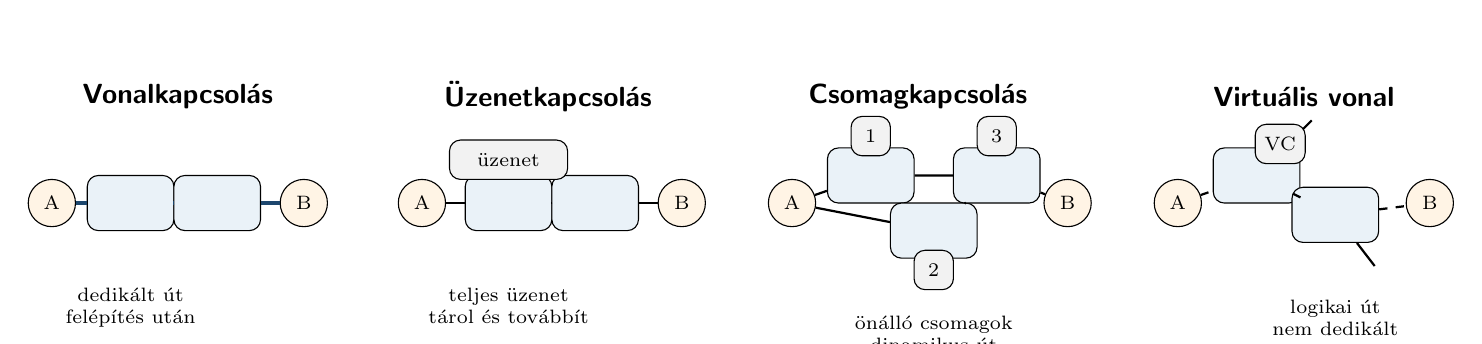
\begin{tikzpicture}[font=\scriptsize]
  \tikzset{host/.style={draw, circle, fill=warnbg, minimum size=6mm, inner sep=0pt},
           sw/.style={draw, rounded corners, fill=lightaccent, minimum width=11mm, minimum height=7mm, align=center},
           data/.style={draw, rounded corners, fill=black!5, minimum height=5mm, align=center},
           link/.style={draw, thick}}

  \begin{scope}[xshift=0cm]
    \node[font=\bfseries\sffamily] at (1.6,1.35) {Vonalkapcsolás};
    \node[host] (ca) at (0,0) {A};
    \node[sw] (c1) at (1,0) {};
    \node[sw] (c2) at (2.1,0) {};
    \node[host] (cb) at (3.2,0) {B};
    \draw[link, accent!90!black, line width=1.2pt] (ca) -- (c1) -- (c2) -- (cb);
    \node[below=6mm of c1, align=center] {dedikált út\\felépítés után};
  \end{scope}

  \begin{scope}[xshift=4.7cm]
    \node[font=\bfseries\sffamily] at (1.6,1.35) {Üzenetkapcsolás};
    \node[host] (ma) at (0,0) {A};
    \node[sw] (m1) at (1.1,0) {};
    \node[sw] (m2) at (2.2,0) {};
    \node[host] (mb) at (3.3,0) {B};
    \draw[link] (ma) -- (m1) -- (m2) -- (mb);
    \node[data, minimum width=15mm] at (1.1,0.55) {üzenet};
    \node[below=6mm of m1, align=center] {teljes üzenet\\tárol és továbbít};
  \end{scope}

  \begin{scope}[xshift=9.4cm]
    \node[font=\bfseries\sffamily] at (1.6,1.35) {Csomagkapcsolás};
    \node[host] (pa) at (0,0) {A};
    \node[sw] (p1) at (1.0,0.35) {};
    \node[sw] (p2) at (1.8,-0.35) {};
    \node[sw] (p3) at (2.6,0.35) {};
    \node[host] (pb) at (3.5,0) {B};
    \draw[link] (pa) -- (p1) -- (p3) -- (pb);
    \draw[link] (pa) -- (p2) -- (p3);
    \node[data, minimum width=5mm] at (1.0,0.85) {1};
    \node[data, minimum width=5mm] at (1.8,-0.85) {2};
    \node[data, minimum width=5mm] at (2.6,0.85) {3};
    \node[below=6mm of p2, align=center] {önálló csomagok\\dinamikus út};
  \end{scope}

  \begin{scope}[xshift=14.3cm]
    \node[font=\bfseries\sffamily] at (1.6,1.35) {Virtuális vonal};
    \node[host] (va) at (0,0) {A};
    \node[sw] (v1) at (1,0.35) {};
    \node[sw] (v2) at (2,-0.15) {};
    \node[host] (vb) at (3.2,0) {B};
    \draw[link, dashed] (va) -- (v1) -- (v2) -- (vb);
    \draw[link] (v1) -- ++(0.7,0.7);
    \draw[link] (v2) -- ++(0.5,-0.65);
    \node[data, minimum width=5mm] at (1.3,0.75) {VC};
    \node[below=6mm of v2, align=center] {logikai út\\nem dedikált};
  \end{scope}
\end{tikzpicture}%
}
\caption{Kapcsolási technikák leegyszerűsített összehasonlítása}
\label{fig:zv22_kapcsolastechnika}
\end{figure}


\section{Rétegezett hálózati architektúra}

\subsection{Miért használunk rétegeket?}

A hálózatok bonyolult rendszerek. Egyetlen kommunikáció során meg kell oldani a fizikai jelátvitelt, a hibák felismerését, a csomagok továbbítását, az útválasztást, a végpontok közötti megbízhatóságot, a formátumkezelést és az alkalmazási protokollokat. Ezt áttekinthetőbbé teszi a \textbf{rétegezés}.

Egy \textbf{réteg} jól definiált szolgáltatásokat nyújt a fölötte lévő rétegnek, és elrejti a szolgáltatás megvalósításának részleteit. A fölötte lévő rétegnek nem kell tudnia, hogy az alsóbb réteg pontosan milyen kódolást, útválasztást vagy hibajavítást használ, csak az interfészen keresztül elérhető szolgáltatásokat látja.

A rétegezés előnyei:

\begin{itemize}
  \item a bonyolult rendszer kisebb, jól definiált részekre bontható;
  \item egy réteg megvalósítása cserélhető, ha az interfész és a szolgáltatás változatlan marad;
  \item különböző gyártók és rendszerek könnyebben együttműködhetnek;
  \item a protokollok és funkciók szabványosíthatók;
  \item a hibakeresés és a tanulás is áttekinthetőbbé válik.
\end{itemize}

\begin{figure}[htbp]
\centering
\resizebox{0.96\textwidth}{!}{%
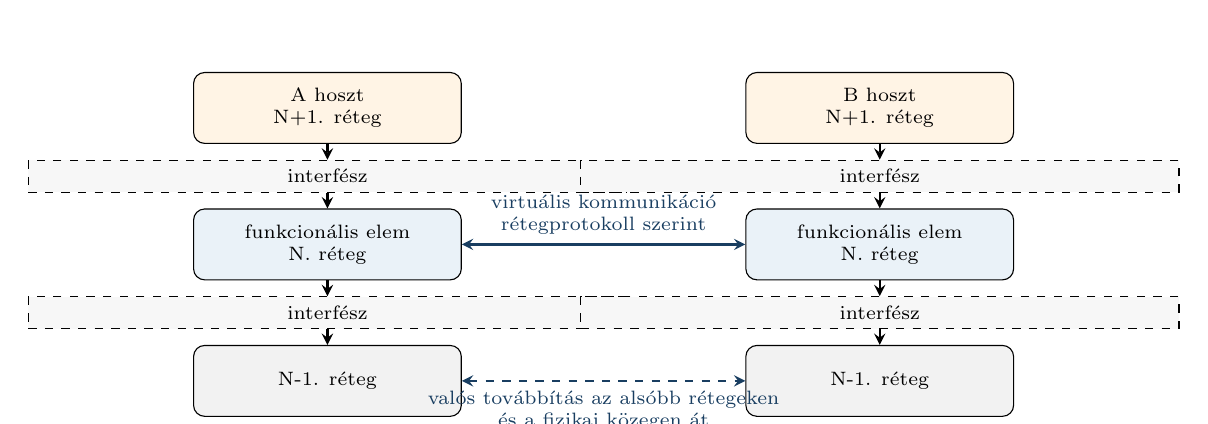
\begin{tikzpicture}[font=\scriptsize, node distance=8mm]
  \tikzset{layerbox/.style={draw, rounded corners, minimum width=34mm, minimum height=9mm, align=center},
           iface/.style={draw, dashed, minimum width=76mm, minimum height=4mm, align=center, fill=black!3},
           vcomm/.style={<->, >=stealth, thick, accent!80!black},
           realcomm/.style={->, >=stealth, thick}}

  \node[layerbox, fill=warnbg] (a3) {A hoszt\\N+1. réteg};
  \node[iface, below=2mm of a3] (ai32) {interfész};
  \node[layerbox, fill=lightaccent, below=2mm of ai32] (a2) {funkcionális elem\\N. réteg};
  \node[iface, below=2mm of a2] (ai21) {interfész};
  \node[layerbox, fill=black!5, below=2mm of ai21] (a1) {N-1. réteg};

  \node[layerbox, fill=warnbg, right=36mm of a3] (b3) {B hoszt\\N+1. réteg};
  \node[iface, below=2mm of b3] (bi32) {interfész};
  \node[layerbox, fill=lightaccent, below=2mm of bi32] (b2) {funkcionális elem\\N. réteg};
  \node[iface, below=2mm of b2] (bi21) {interfész};
  \node[layerbox, fill=black!5, below=2mm of bi21] (b1) {N-1. réteg};

  \draw[realcomm] (a3) -- (ai32);
  \draw[realcomm] (ai32) -- (a2);
  \draw[realcomm] (a2) -- (ai21);
  \draw[realcomm] (ai21) -- (a1);
  \draw[realcomm] (b3) -- (bi32);
  \draw[realcomm] (bi32) -- (b2);
  \draw[realcomm] (b2) -- (bi21);
  \draw[realcomm] (bi21) -- (b1);

  \draw[vcomm] (a2.east) -- node[above, align=center]{virtuális kommunikáció\\rétegprotokoll szerint} (b2.west);
  \draw[vcomm, dashed] (a1.east) -- node[below, align=center]{valós továbbítás az alsóbb rétegeken\\és a fizikai közegen át} (b1.west);
\end{tikzpicture}%
}
\caption{Rétegezett hálózati architektúra: virtuális és valós kommunikáció}
\label{fig:zv22_retegzett_architektura}
\end{figure}


\subsection{Protokoll, interfész és szolgáltatás}

A rétegezett modell három alapfogalmát vizsgán érdemes pontosan elválasztani.

A \textbf{protokoll} azonos rétegű, különböző gépeken lévő társelemek közötti kommunikáció szabályrendszere. Meghatározza, milyen formátumú adategységeket küldenek, milyen mezők vannak bennük, milyen sorrendben történnek az események, és mit jelentenek az egyes üzenetek.

Az \textbf{interfész} két szomszédos réteg között található. Leírja, hogy a felső réteg milyen műveletekkel és paraméterekkel kérhet szolgáltatást az alsó rétegtől, illetve milyen eredményt kap vissza.

A \textbf{szolgáltatás} az, amit egy réteg a fölötte lévő réteg számára biztosít. Röviden: a szolgáltatás a kívülről látható képesség, a protokoll pedig az a szabályrendszer, amellyel a társelemek ezt megvalósítják.

\subsection{Társelemek, virtuális és valós kommunikáció}

A \textbf{társelemek} különböző gépeken azonos rétegben lévő funkcionális elemek. Például az egyik gép szállítási rétege logikailag a másik gép szállítási rétegével kommunikál. Ezt nevezzük \textbf{virtuális kommunikációnak}, mert a két réteg között úgy tekintjük, mintha közvetlen kapcsolat lenne.

A valóságos adatmozgás azonban másként történik: az adat a küldő oldalon rétegről rétegre lefelé halad, eljut a fizikai közegre, majd a fogadó oldalon rétegről rétegre felfelé halad. Az alsóbb rétegek fejléceket, esetleg utótagokat adnak hozzá; a fogadó oldalon ezek lekerülnek és értelmeződnek. Ezt nevezik beágyazásnak vagy enkapszulációnak.

\subsection{Szolgáltatástípusok és primitívek}

A hálózati szolgáltatás lehet \textbf{összeköttetés-alapú} vagy \textbf{összeköttetésmentes}. Összeköttetés-alapú szolgáltatásnál először kapcsolatot építenek fel, ezután történik az adatátvitel, majd a kapcsolat bontása. Ez sorrendhelyesebb, állapottartóbb szemlélet. Összeköttetésmentes szolgáltatásnál minden adategység tartalmazza a célcímet, és egymástól függetlenül továbbítódik; ilyen a datagram jellegű működés.

Mindkét szolgáltatástípus lehet nyugtázott vagy nyugtázatlan. Nyugtázott szolgáltatásnál a küldő visszajelzést kap arról, hogy a kérés vagy adatátvitel megtörtént. Nyugtázatlan szolgáltatásnál kisebb lehet a többletterhelés, de a megbízhatóságot más rétegnek vagy az alkalmazásnak kell biztosítania.

Az OSI szemléletben a szolgáltatásokat primitívek írhatják le:

\begin{itemize}
  \item \textbf{kérés} (request): a felsőbb réteg szolgáltatást kér;
  \item \textbf{bejelentés} (indication): a réteg jelzi a felsőbb rétegnek, hogy esemény történt;
  \item \textbf{válasz} (response): a felsőbb réteg válaszol a bejelentésre;
  \item \textbf{megerősítés} (confirm): a kérő fél visszajelzést kap az eredményről.
\end{itemize}

\section{Az ISO--OSI hivatkozási modell}

\subsection{A referencia modell szerepe}

Az \textbf{ISO--OSI modell} a nyílt rendszerek összekapcsolásának hivatkozási modellje. Az ISO nemzetközi szabványosítási szemléletében készült, és hét rétegben írja le a hálózati kommunikáció funkcióit.

Fontos vizsgamondat, hogy az OSI modell \textbf{referencia modell}, nem pedig konkrét hálózati architektúra. Nem ad meg teljes konkrét protokollkészletet, és nem ír elő egyetlen konkrét implementációt. Azt határozza meg, hogy milyen feladatokat érdemes külön rétegekbe szervezni.

A rétegek kialakításának fő szempontjai:

\begin{itemize}
  \item minden réteg más absztrakciós szintet képviseljen;
  \item a rétegeknek jól definiált feladataik legyenek;
  \item a rétegek között minimális és tiszta információcsere történjen;
  \item a rétegek száma ne legyen túl kevés, mert akkor túl sok feladat kerülne egy rétegbe;
  \item a rétegek száma ne legyen túl sok, mert akkor a modell nehezen kezelhető lenne.
\end{itemize}

\begin{figure}[htbp]
\centering
\resizebox{0.92\textwidth}{!}{%
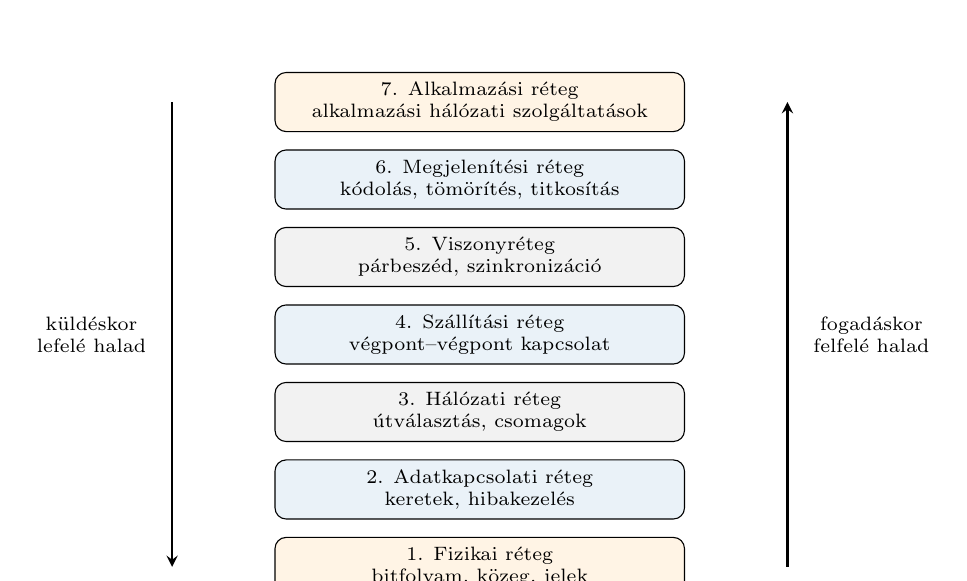
\begin{tikzpicture}[font=\scriptsize, node distance=2.2mm]
  \tikzset{osilayer/.style={draw, rounded corners, minimum width=52mm, minimum height=7.5mm, align=center}}
  \node[osilayer, fill=warnbg] (l7) {7. Alkalmazási réteg\\alkalmazási hálózati szolgáltatások};
  \node[osilayer, fill=lightaccent, below=of l7] (l6) {6. Megjelenítési réteg\\kódolás, tömörítés, titkosítás};
  \node[osilayer, fill=black!5, below=of l6] (l5) {5. Viszonyréteg\\párbeszéd, szinkronizáció};
  \node[osilayer, fill=lightaccent, below=of l5] (l4) {4. Szállítási réteg\\végpont--végpont kapcsolat};
  \node[osilayer, fill=black!5, below=of l4] (l3) {3. Hálózati réteg\\útválasztás, csomagok};
  \node[osilayer, fill=lightaccent, below=of l3] (l2) {2. Adatkapcsolati réteg\\keretek, hibakezelés};
  \node[osilayer, fill=warnbg, below=of l2] (l1) {1. Fizikai réteg\\bitfolyam, közeg, jelek};

  \coordinate (sendTop) at ([xshift=-13mm]l7.west);
  \coordinate (sendBottom) at ([xshift=-13mm]l1.west);
  \coordinate (recvBottom) at ([xshift=13mm]l1.east);
  \coordinate (recvTop) at ([xshift=13mm]l7.east);
  \draw[arrow] (sendTop) -- (sendBottom) node[midway, left=2mm, align=center]{küldéskor\\lefelé halad};
  \draw[arrow] (recvBottom) -- (recvTop) node[midway, right=2mm, align=center]{fogadáskor\\felfelé halad};

\end{tikzpicture}%
}
\caption{Az ISO--OSI modell hét rétege és az adat útja}
\label{fig:zv22_osi_modell}
\end{figure}


\subsection{Az alsó rétegek: fizikai, adatkapcsolati, hálózati}

Az \textbf{1. fizikai réteg} a bitek kommunikációs csatornán való átviteléért felel. Ide tartozik a jelek elektromos, optikai vagy rádiós reprezentációja, a csatlakozók fizikai kialakítása, a közeg tulajdonságai, az adatátviteli irányok, valamint a mechanikai, villamos, funkcionális és eljárási specifikációk. A fizikai réteg PDU-ja szemléletesen a bitfolyam.

A \textbf{2. adatkapcsolati réteg} a fizikai közeg fölött keretekkel dolgozik. Fő feladata a keretképzés és kerethatárolás, hibák ellenőrzése és javítása, adatfolyam-vezérlés, valamint üzenetszórásos közeg esetén a közeghozzáférés szabályozása. Az adatkapcsolati réteg gyakran két alrétegre bontható: LLC és MAC szemléletre, ahol a MAC a közeghez való hozzáféréssel foglalkozik.

A \textbf{3. hálózati réteg} csomagok továbbításával és útválasztással foglalkozik. Feladata a forrástól a célig vezető út meghatározása, a csomagok továbbítása köztes csomópontokon keresztül, a torlódás kezelése és heterogén hálózatok összekapcsolása. Az útválasztás lehet statikus vagy dinamikus.

\subsection{A középső és felső rétegek: szállítási, viszony, megjelenítési, alkalmazási}

A \textbf{4. szállítási réteg} valódi végpont--végpont réteg. A fölötte lévő rétegektől kapott adatokat szükség esetén feldarabolja, majd a fogadó oldalon összeállítja. Feladata lehet az összeköttetések kezelése, multiplexálás, adatfolyam-vezérlés, hibakezelés és megbízható sorrendhelyes átvitel biztosítása.

Az \textbf{5. viszonyréteg} felhasználói viszonyokat és párbeszédeket kezel különböző gépek között. Feladata a párbeszédszervezés, a szinkronizáció és a kölcsönhatás menedzselése. Nagyobb adatátvitel esetén például szinkronizációs pontokkal segítheti, hogy hiba után ne kelljen mindent elölről kezdeni.

A \textbf{6. megjelenítési réteg} az átviendő információ szintaktikájával és szemantikájával foglalkozik. Tipikus feladata a kódoláskonverzió, adattípus- és formátumkezelés, tömörítés és titkosítás. Lényege, hogy a különböző rendszerek eltérő belső adatábrázolása mellett is értelmezhető legyen az információ.

A \textbf{7. alkalmazási réteg} a felhasználói alkalmazásokhoz közel álló hálózati szolgáltatásokat tartalmazza. Példák: fájlátvitel, elektronikus levelezés, webes szolgáltatások, távoli bejelentkezés, címtárszolgáltatások, adatbázis-elérés vagy nyomtatási szolgáltatások. Itt jelennek meg azok a protokollok, amelyeket a felhasználói programok közvetlenebbül használnak.

\begin{center}
\begin{tabularx}{\textwidth}{L{24mm}L{26mm}X}
\toprule
\textbf{Réteg} & \textbf{Tipikus PDU} & \textbf{Fő feladatok} \\
\midrule
7. Alkalmazási & Üzenet & Felhasználói és alkalmazási hálózati szolgáltatások, például fájlátvitel, elektronikus levelezés, web, távoli bejelentkezés. \\
6. Megjelenítési & Üzenet & Adatformátumok kezelése, kódoláskonverzió, tömörítés, titkosítás, az információ szintaktikája és szemantikája. \\
5. Viszony & Üzenet & Kommunikációs viszonyok létrehozása és kezelése, párbeszédszervezés, szinkronizáció, kölcsönhatás-kezelés. \\
4. Szállítási & Szegmens / datagram & Valódi végpont--végpont adatátvitel, tördelés és összeállítás, multiplexálás, hibakezelés, adatfolyam-vezérlés. \\
3. Hálózati & Csomag & Útválasztás, forrás és cél közötti továbbítás, torlódásvezérlés, heterogén hálózatok összekapcsolása. \\
2. Adatkapcsolati & Keret & Keretképzés, kerethatárolás, hibadetektálás és javítás, adatfolyam-vezérlés, szükség esetén közeghozzáférés. \\
1. Fizikai & Bitfolyam & Bitek átvitele a kommunikációs csatornán, jelek, csatlakozók, közeg, adatátviteli irányok és fizikai paraméterek. \\
\bottomrule
\end{tabularx}

\end{center}

\section{OSI szemlélet alkalmazása és PDU-k}

\subsection{Beágyazás és címzés}

Amikor egy alkalmazás adatot küld, az adat a felső rétegektől az alsó rétegek felé halad. Minden réteg a saját céljaihoz szükséges vezérlőinformációt adhat hozzá, például fejléc formájában. A fogadó oldalon a rétegek fordított sorrendben dolgoznak: az alsóbb réteg értelmezi és eltávolítja a saját vezérlőinformációját, majd az adatot átadja a felsőbb rétegnek.

A különböző rétegek eltérő címzési és azonosítási formákat használhatnak. Az adatkapcsolati rétegben például fizikai vagy MAC-címekről beszélhetünk, a hálózati rétegben logikai hálózati címekről, a szállítási rétegben pedig portokról vagy végpont-azonosítókról.

\subsection{Rétegek közötti felelősségmegosztás}

A rétegek nem elszigetelt témák, hanem egymásra épülő felelősségi szintek. A fizikai réteg csak biteket továbbít, de nem tudja, hogy azok milyen alkalmazási üzenetet alkotnak. Az adatkapcsolati réteg helyi kereteket kezel, a hálózati réteg már több hálózaton át vezető útvonalat választhat, a szállítási réteg pedig a végpontok közötti szolgáltatás minőségét javíthatja.

Ezért vizsgán nem elég csak felsorolni a hét réteget. Röviden meg kell mutatni azt is, hogy alulról felfelé haladva egyre absztraktabb szolgáltatásokat kapunk: fizikai jelátvitelből helyi keretátvitel, abból csomagtovábbítás, abból végpont--végpont kommunikáció, végül alkalmazási szolgáltatás lesz.

\section{Gyakori vizsgahibák és összefoglalás}

\subsection{Gyakori félreértések}

\begin{itemize}
  \item \textbf{Az OSI modell és a TCP/IP összekeverése.} A 22. tételben az OSI referencia modell a lényeg; konkrét TCP/IP összevetés inkább a későbbi hálózatos tételekhez tartozik.
  \item \textbf{Referencia modell és architektúra azonosítása.} Az OSI nem konkrét implementáció, hanem funkcionális rétegmodell.
  \item \textbf{Protokoll és szolgáltatás összekeverése.} A szolgáltatás azt mondja meg, mit nyújt egy réteg, a protokoll azt, hogyan kommunikálnak a társelemek.
  \item \textbf{Fizikai és logikai kommunikáció összekeverése.} A társelemek kommunikációja logikai/virtuális; a valós adatmozgás a rétegeken keresztül és a fizikai közegen történik.
  \item \textbf{Vonalkapcsolás és virtuális vonalkapcsolás azonosítása.} A virtuális vonal logikai útvonal, de nem dedikált fizikai vonal.
  \item \textbf{Üzenetkapcsolás és csomagkapcsolás összemosása.} Üzenetkapcsolásnál teljes üzeneteket tárolnak és továbbítanak, csomagkapcsolásnál kisebb, korlátos méretű csomagok mozognak.
  \item \textbf{Topológia puszta rajzként kezelése.} A topológia hatással van a hibaterjedésre, redundanciára, költségre és menedzselhetőségre.
  \item \textbf{A rétegek sorrendjének eltévesztése.} Alulról: fizikai, adatkapcsolati, hálózati, szállítási, viszony, megjelenítési, alkalmazási.
\end{itemize}

\subsection{Rövid vizsgaválasz-minta}

\begin{summarybox}
A számítógép-hálózat autonóm számítógépek kommunikációs alrendszerrel összekapcsolt rendszere. Célja az erőforrások megosztása, a megbízhatóság és gazdaságosság növelése, valamint új kommunikációs szolgáltatások biztosítása. Méret szerint beszélhetünk LAN, MAN, WAN és világméretű összekapcsolt hálózatokról. Kapcsolati szerkezet szerint megkülönböztetünk pont--pont hálózatokat és üzenetszórásos csatornára épülő hálózatokat. Topológia szerint gyakori a sín, csillag, gyűrű, fa, teljes/részleges háló és szabálytalan szerkezet. Kapcsolástechnika alapján a vonalkapcsolás dedikált kapcsolatot épít fel, az üzenetkapcsolás teljes üzeneteket tárol és továbbít, a csomagkapcsolás az üzeneteket kisebb csomagokra bontja, a virtuális vonalkapcsolás pedig csomagkapcsolt működés mellett előre kialakított logikai útvonalat használ. A hálózati rendszereket rétegekbe szervezzük: egy réteg szolgáltatást nyújt a fölötte lévőnek, protokollal kommunikál a másik gépen lévő társelemével, és interfészen keresztül használja az alatta lévő réteget. Az ISO--OSI modell hét rétegű referencia modell: fizikai, adatkapcsolati, hálózati, szállítási, viszony, megjelenítési és alkalmazási réteg. Nem konkrét protokollkészletet ír elő, hanem a hálózati kommunikáció funkcióit választja szét jól definiált absztrakciós szintekre.
\end{summarybox}

\end{document}
